%%%% ijcai19.tex

\typeout{IJCAI-19 Instructions for Authors}

% These are the instructions for authors for IJCAI-19.

\documentclass{article}
\pdfpagewidth=8.5in
\pdfpageheight=11in
% The file ijcai19.sty is NOT the same than previous years'
\usepackage{ijcai19}

% Use the postscript times font!
\usepackage{times}
\usepackage{soul}
\usepackage{url}
%\usepackage[hidelinks]{hyperref}
\usepackage[utf8]{inputenc}
\usepackage[small]{caption}
\usepackage{graphicx}
\usepackage{subfigure}
\usepackage{amsmath}
\usepackage{booktabs}
\usepackage{algorithm}
\usepackage{algorithmic}
\usepackage{multirow}
\usepackage{array}
\urlstyle{same}
% the following package is optional:
%\usepackage{latexsym} 

\usepackage{bm}
\newcommand{\PRN}{{\sf PRN}}
\newcommand{\etal}{{\it et al.}}

% Following comment is from ijcai97-submit.tex:
% The preparation of these files was supported by Schlumberger Palo Alto
% Research, AT\&T Bell Laboratories, and Morgan Kaufmann Publishers.
% Shirley Jowell, of Morgan Kaufmann Publishers, and Peter F.
% Patel-Schneider, of AT\&T Bell Laboratories collaborated on their
% preparation.

% These instructions can be modified and used in other conferences as long
% as credit to the authors and supporting agencies is retained, this notice
% is not changed, and further modification or reuse is not restricted.
% Neither Shirley Jowell nor Peter F. Patel-Schneider can be listed as
% contacts for providing assistance without their prior permission.

% To use for other conferences, change references to files and the
% conference appropriate and use other authors, contacts, publishers, and
% organizations.
% Also change the deadline and address for returning papers and the length and
% page charge instructions.
% Put where the files are available in the appropriate places.

% \title{Social Relationship Detection using Rules}

\title{Understanding Social Relationship with Person-pair Relations}

% Single author syntax
\author{
    % Sarit Kraus
    % \affiliations
    % Department of Computer Science, Bar-Ilan University, Israel \emails
    % pcchair@ijcai19.org
    \#229
}

% Multiple author syntax (remove the single-author syntax above and the \iffalse ... \fi here)
% Check the ijcai19-multiauthor.tex file for detailed instructions
\iffalse
\author{
First Author$^1$
\and
Second Author$^2$\and
Third Author$^{2,3}$\And
Fourth Author$^4$
\affiliations
$^1$First Affiliation\\
$^2$Second Affiliation\\
$^3$Third Affiliation\\
$^4$Fourth Affiliation
\emails
\{first, second\}@example.com,
third@other.example.com,
fourth@example.com
}
\fi

\begin{document}

\maketitle

\begin{abstract}
% Social relationships play a very important role in social network. Social relationship understanding has attracted increasing attention, typically, which can help to understand the behavior of humen in our daily life. Previous social relationship understanding models focused too much on relationships between the same pair and ignore the interplay of different relationships in the same scene.  We found that the interaction between the relationships in the same scene plays an important role in the understanding of social relations and we can make meanful use of rules during inference. This paper proposes a novel model named {\it SRDR} which incorporates rules seamlessly into the deep learning model named {\it SR}  to solve the social relationship understanding problem. It formulates inference as an integer linear programming (ILP) problem, with the objective function generated from {\it SR} and the constraints translated from rules. By incorporating rules, our approach can greatly reduce the solution space and significantly improve the inference accuracy of social relationship understanding models. Experimental results on two classic data sets show that our approach significantly outperforms state-of-the-art  models in social relationship understanding, which justifies the significance of incorporating rules seamlessly into the deep learning model in social relationship understanding task.

Social relationships understanding is to infer the social relations among people from images and videos, which has attracted increasing attention in computer vison recently. A great progress has been made since the rise of deep learning. However, they mostly focus on the facial attributes or contextual object cues without taking into account the interaction among person pairs. Motivated by scene graph generation, we carefully analyzed the datasets and found the social relations in a still image always have high semantic relevance. For instance, if two person pair in an image are {\it Friends}, then the third one is always friends or at least other intimate relations but not {\it No Relation}. Therefore, to capture this interaction cues, we propose a novel end-to-end trainable Person-Pair Relation Network (\PRN) using standard RNNs, a graph inference network that learns iteratively to improve its predictions via message passing among person pair nodes. Extensive experiments on PISC and PIPA-Relation show the superiority of our method over previous methods. 

\end{abstract}

\section{Introduction}
Social relationships are closely related to our daily life \cite{DBLP:conf/wacv/BarrCBF14}. After understanding the social relationship between the person pair, we can easily explain their behavior. For machines, only when they fully understand the social relationships, can they further understand and infer the human behavior in our social life, so as to make a better response. In addition, we often leave traces that capture social relationships in many medias and we not only want the machines to be proficient at their task, but also enable them to blend in and
act appropriately in different situations \cite{DBLP:conf/cvpr/SunSF17}. In short, social relationship detection task is very significant in many ways. In our work, we aim to address the social relationship detection task for every picture where each picture represents a scene. 

However, to solve the social relationship detection task is not so simple. For a giving picture, detecting the social relationships of all the person pair is a difficult task. The models need to be adapted to different scenes and context information to make right judgments.  \cite{DBLP:conf/cvpr/SunSF17} use the information of head region, body region and human attributes to predict the person-pair's social relationship separately. \cite{DBLP:conf/iccv/LiWZK17} make use of the pair of people in question and region proposals and allocate attention to each region to detect the social relationship of each person pair. \cite{DBLP:conf/ijcai/WangCRYCL18} takes advantage of the message propagation between person pair social relationship and the object  semantic regions to solve the problem. The biggest problem of these models is that they all only detect one relationship per step which will cause that different social relationships in the same scene cannot interact with each other. Social relationships in the same scene are strongly linked but the previous models have ignored this important information.

\vspace*{-1mm}
\begin{figure}[htpb]
	\centering
	%	\includegraphics[width=0.48 \textwidth, trim=10 10 10 80,clip]{./pic/example_new.pdf}
	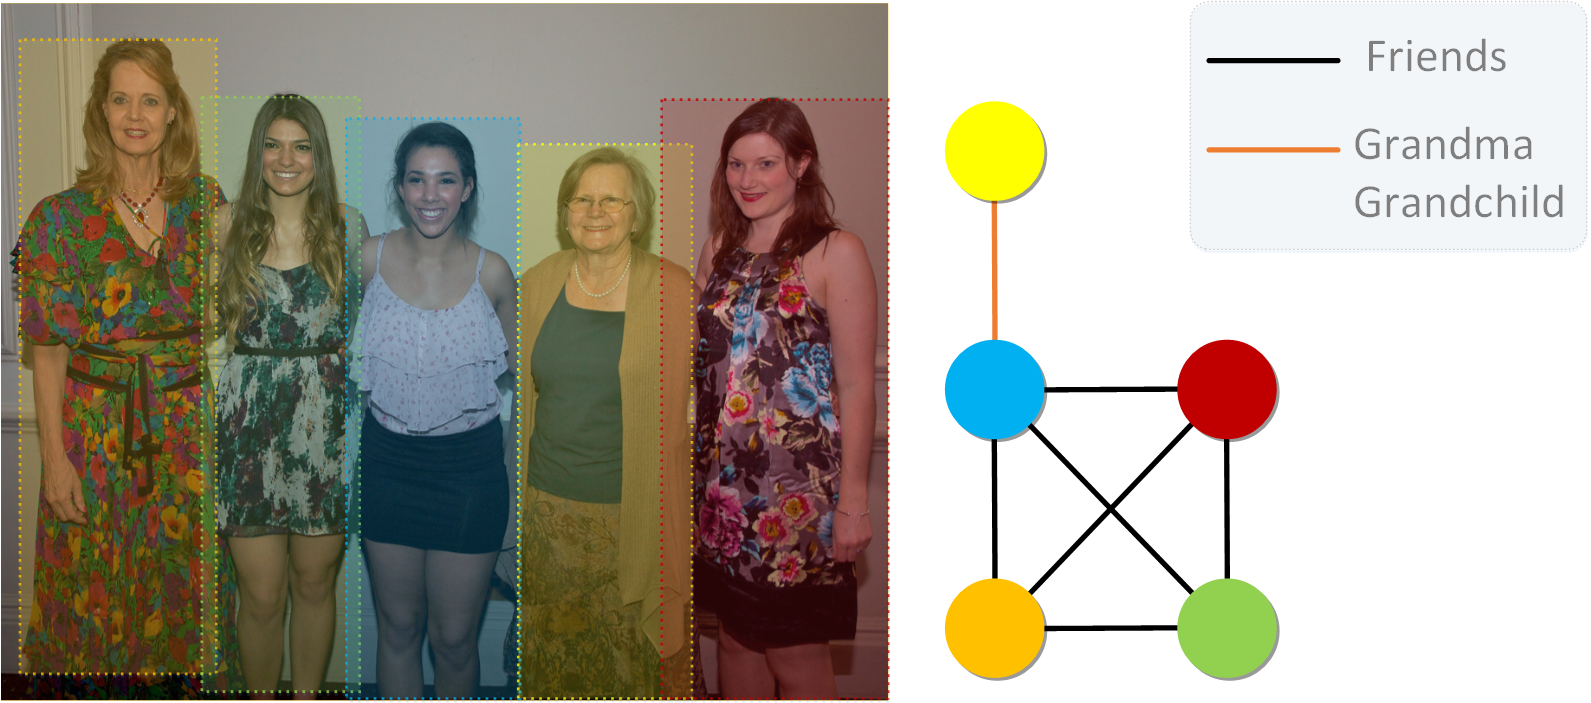
\includegraphics[width=0.48 \textwidth,clip]{./pic/example.png}
	%\hspace{0.02\textwidth}
	%\vspace*{-0.08cm}
  \caption{An example image and its social relation graph from PIPA-relation. The person in various color boxes corresponds to the same color node in the graph. An edge linked to two nodes denotes the social relation between them. There are many examples with stable social relation in whole dataset and the detail statistic is in Sec. \ref{section:dataset_anaysis}.}
	\vspace*{-3.5mm}
	\label{fig:example}
\end{figure}

As one example from PIPA-relation \cite{DBLP:conf/cvpr/SunSF17} shown in Figure \ref{fig:example}, the social relationship of six person pairs is {\it Friends} except one is {\it Grandma\_grandchild}, which is mostly a group of friends. Intuitively, if we want to infer the social relationship of a person pair and already know several others with same relationships such as Friends, then the person pair has a high probability of being Friends. Therefore, the cues of contextual social relationships play an important role in social relationships understanding.

However, the biggest issue of the task is that it is not as simple as people directly to judge the result. We need to design the mechanism of the interaction between social relationships and effectively model the mechanism. The other issue is how to use less effective information to model the interaction machanism and get the better result. For example, whether to introduce the information of the objects in scene has also became an important consideration for us.

To address this problem, we propose a novel end-to-end trainable Person-Pair Relation Network (\PRN) which makes good use of the information of social relationship interaction in the same scene. \PRN \ consists of 3 parts:  \emph{feature extraction module}, \emph{message pooling module} and \emph{message passing module}. In the feature extraction module, we use a Resnet\cite{DBLP:conf/cvpr/HeZRS16} to extract features of each person and another Resnet to extract features of the person pairs in the image. In this module, the position of each person is also taken into account. In the message pooling module, we use a attention mechanism to make all the social relationships interact with each other well and the outout of this module will be considered as the inputs of the GRU which is in the next module. In the message passing module,  we use the RNNs contained GRU to make the social relationship message passing proceed iteratively. As the model proceeding, this module and the message pooling module will have an interaction and make the overall interaction mechanism better. We use the hidden states of the last GRU as the social relationship detection results of the scene.

We evaluate our model in classic datasets: PIPA-Relation dataset and PISC dataset. The experiment results verify the superiority of our model over previous methods. Specifically, our contributions are as follows:
\begin{itemize}
	\item To our best knowledge, it is the first attempt to introduce the interaction of social relationships in the same scene on the social relationship detection task;
	\item We design a novel interaction mechanism to model the interaction of social relationships in the same scene which gets the best result in this task;
	\item We analyze and verify that the role played by objects in the scene is not very big which is a very novel idea in the social relationship detection task.
\end{itemize}


\section{Related Work}

\subsection{Social Relationship Understanding}
% Introduce social relationship understanding including \cite{DBLP:conf/aaai/GuoWWWG18}, \cite{DBLP:conf/iccv/LiWZK17}, \cite{DBLP:conf/ijcai/WangWG15} and \cite{DBLP:conf/ijcai/WangCRYCL18}.

The foundation of social network is the social relationships understanding, an important multidisciplinary problem that has attracted increasing attention in computer vision recently. A much number of studies that aim to infer social relationships from images \cite{DBLP:conf/ijcai/WangWG15,DBLP:conf/iccv/LiWZK17,DBLP:conf/ijcai/WangCRYCL18,DBLP:conf/eccv/WangGLF10,DBLP:conf/iccv/ZhangLLT15} and videos \cite{DBLP:conf/eccv/DingY10,DBLP:conf/cvpr/RamanathanY013,DBLP:journals/ivc/VinciarelliPB09} have been made since the rise of deep learning. For instance, motivated by psychological sudies, \cite{DBLP:conf/iccv/ZhangLLT15} and \cite{DBLP:conf/iccv/DibekliogluSG13} exploit social relationships based on facial attributs such as expression and head pose, and affective behaviour analysis. Besides, \cite{DBLP:conf/iccv/LiWZK17} and \cite{DBLP:conf/ijcai/WangCRYCL18} discover that contextual cues around people play a significant role in social realtionship infering. Concretely, \cite{DBLP:conf/iccv/LiWZK17} proposed a dual-glance model for social relationship, where the first glance makes a coarse relationship prediction for a given person pair and then the second one refines the prediction by using the objects around the pair. \cite{DBLP:conf/ijcai/WangCRYCL18} constructed a semantic-aware knowledge graph and employed Gated Graph Neural Network (GGNN) \cite{DBLP:journals/tomccap/LiSKJZW15} to integrate the graph into the Graph Reasoning Model (GRM), a graph reasoning network where a proper message propagation and graph attention mechanism are introduced to explore the interaction between person pair and the contextual objects.

Unlike the aforementioned works which mainly focus on facial attributs or contextual object cues, we studied the two classic datasets PISC \cite{DBLP:conf/iccv/LiWZK17} and PIPA-relation \cite{DBLP:conf/cvpr/SunSF17} in Sec. \ref{section:dataset_anaysis} and found the social relationships in a still image are always stable. Based on this discovery, we designed a novel end-to-end trainable Person-Pair Relation Network (PRN), a graph inference network to capture this semantic relevance cues via message passing among person pair nodes.

\subsection{Message Passing}%
Graph inference is a kind of form of message passing and Conditional Random Fields (CRF) have been used extensively in this field. Johnson \etal \ used CRF to infer scene graph grounding distributions for image retrieval \cite{DBLP:conf/cvpr/JohnsonKSLSBL15}. Yatskar \etal \ use a deep CRF model to propose situation-driven object and action prediction\cite{DBLP:conf/cvpr/YatskarZF16} . Danfei Xu \etal \ use the GRU-RNNs to solve the scene graph generation problem iteratively\cite{DBLP:conf/cvpr/XuZCF17}. Our work is related to Graph-LSTM \cite{DBLP:conf/eccv/LiangSFLY16} and  the work of  Danfei Xu \etal \cite{DBLP:conf/cvpr/XuZCF17} which formulate the message passing problem using RNN models. Danfei Xu \etal \cite{DBLP:conf/cvpr/XuZCF17} design primal graph and dual graph in their model while we just simplify the model and just use one graph to make social relationship messages to pool and achieve a better result. As what Danfei Xu \etal \cite{DBLP:conf/cvpr/XuZCF17} have done, our model iteratively refines the social relationship predictions through relationship message passing in the scene, whereas the Structural RNN model only makes one-time predictions along the temporal dimension, and thus cannot refine its past predictions\cite{DBLP:conf/cvpr/XuZCF17}.
\vspace*{-3mm}
\begin{figure*}[htpb]
	\centering
	%	\includegraphics[width=0.48 \textwidth, trim=10 10 10 80,clip]{./pic/example_new.pdf}
	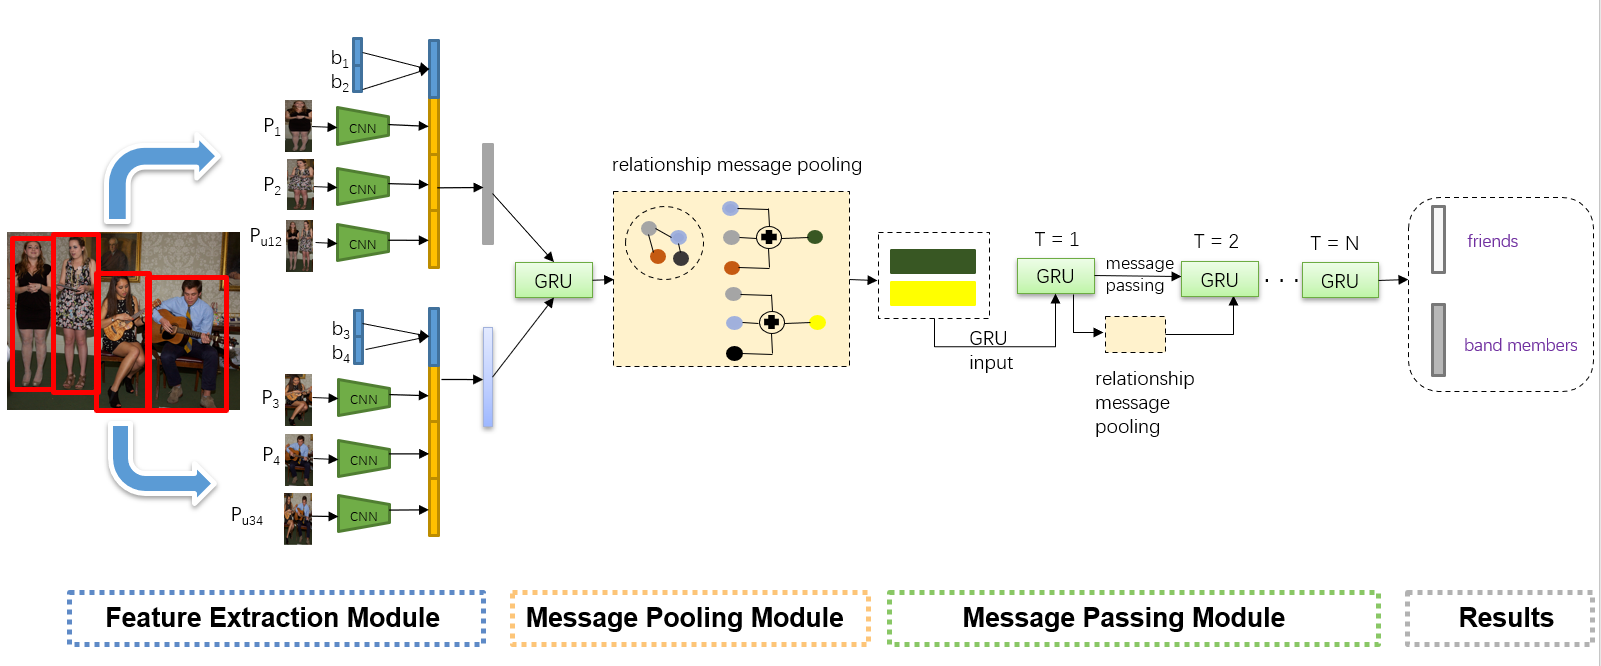
\includegraphics[width=0.96 \textwidth,clip]{./pic/model_2.png}
	%\hspace{0.02\textwidth}
	%\vspace*{-0.08cm}
	\caption{An illustration of our \PRN . The model first extracts the features of each person and person pairs in the Feature Extraction Module. $P_i$ denotes the $i$th person and $P_{uij}$ denotes the union region of $i$th person and $j$th person. $b_i$ denotes the position of the $i$th person. In the Message Pooling Module, a message pooling function computes relationship messages that are passed to the node GRU in the next iteration from the hidden states. The $\oplus$ symbol denotes a learnt weighted sum. Then in the Message Passing Module, we iteratively updates the hidden states of the GRUs. We use the hidden states of the GRUs at the last iteration step, to predict the social relationships in the scene.}
	\vspace*{-3.5mm}
	\label{fig:model}
\end{figure*}


\section{PRN \ Model}

\subsection{Overview} \label{section:ov}
In this section, we introduce the proposed person-pair relational network for social relationship understanding. We fomulate the relationships of an image as a \emph{social graph}, each node denotes relationship of a person pair. Then, taking the same approach as GRM\cite{DBLP:conf/ijcai/WangCRYCL18} to extract various features initialize these nodes. Person pair relation  network employs Gated Recurrent Unit\cite{DBLP:conf/ssst/ChoMBB14} to explore the interaction of relationships with each other, and we employ the attention mechanism to adaptively exploit the most relevant nodes. It integrates multiple
component to learn the representations of relationshipes between peoples in an image. 
 The proposed framework is shown in Fig. 2.

\subsection{Feature Extraction Module} \label{section:vs}

Given an image \textbf{I} and the bounding box of peoples, we first crop three patches for each person pair, where the first two cover each person, $\mathbf{p_1}$ and $\mathbf{p_2}$, and one for union region, $\mathbf{p_u}$, that cover the both people and maintains the basic information for recognition. These patches are resized to $224\times224$ pixels and fed into three CNNs, These feature vectors from the last convolutional layer are flattened and concatenated. $\mathbf{p_1}$ and $\mathbf{p_2}$ share the same weights.
In addition, geometry feature of bounding box is complementary to the visual appearance, as the relation $\emph{No Relation}$, which is not easy to learn only from visual feature. We denote the geometry feature of bounding box i as $b_i^{pos}$ = $\{x_i^{min}, y_i^{min},x_i^{max},y_i^{max},area_i\}$  $\in$ $\mathbf{R}^5$, where all the parameters are relative values. These features also concatenated with the CNN features for $p_1,p_2$ and $p_u$ to form a single vector. Finally, both of them are fed into a fully connected layer to produce a 4096-dimension feature vector $v_h$. 


\subsection{Message Passing Module} \label{section:RRNN}
In this subsection, we will talk about how the social relationship message will pass to each other.
In this Message Passing Module, we use the Recurrent Neural Networks(RNNs) to finish the inference of the social relationship detection task. In contrast to Zheng \etal \ \cite{DBLP:conf/iccv/0001JRVSDHT15}, our model use a generic RNN module to compute the hidden states. In addition, we select the best cell Gated Recurrent Units \cite{DBLP:conf/ssst/2014} for RNNs.We use the hidden state of the $t$-th step to denote the relationship node of the current social graph. In addition, the initial hidden state of the GRU is randomly assigned and the rest hidden state inheritance in the hidden state from the previous step. So the relationship node will be updated step by step as the GRU-based RNN going. Besides, the input of the GRU for each step comes from the output of the Message Pooling Module which has completed a social relationship interaction. In particular, the feature vector $v_h$ which comes from Feature Extraction Module will be fed into the first GRU. On the whole, the Message Passing Module can be formulated as follows:
%\vspace{-0.5mm}
\begin{equation}
\begin{split}
\bm{r}_t &=  \sigma(\bm{W}_{r}[\bm{h}_{t-1}, \bm{x}_t]), \\
\bm{z}_t &=  \sigma(\bm{W}_{z}[\bm{h}_{t-1}, \bm{x}_t]), \\
\hat{\bm{h}_t} &= tanh(\bm{W}[\bm{r}_t \odot \bm{h}_{t-1}, \bm{x}_{t}])\\
\bm{h}_t &= (1 - \bm{z}_t) \odot \bm{h}_{t - 1} + \bm{z}_t \odot \hat{\bm{h}_t} \\
\end{split}
\end{equation}
where $\sigma$ and $tanh$ are the logistic sigmoid and hyperbolic tangent functions. In addition, $\odot$ symbol denotes the element-wise multiplication operation. $\bm{r}_t$ denotes the reset gate in $t$ step and $\bm{z}_t$ denotes the update gate at $t$ step. $\bm{W}_r$ and $\bm{W}_z$ denotes weights of reset gate and update gate. $\bm{W}_r$, $\bm{W}_z$ and $\bm{W}$ are trainable parameters. Specially, $\bm{x}_0$ initialized by the output of feature extraction module. At $t$-th step, each GRU takes the previous hidden state $\bm{h}_{t-1}$ and the coming messages $\bm{x}_{t}$ as input, and produce a new hidden state. By the way, $\bm{x}_t$ computed by Message Passing Module. Each node in \emph{social graph} holds the inner state in the corresponding GRU cell. At last, we use the last hidden state of the GRU unit to represent the social relationship of each node and output the results.

\subsection{Message pooling Module} \label{section:mp}

Sec \ref{section:vs} provides a way to solve reasoning problem using RNNs. As each GRU receives multiple incoming messages, we need an aggregation function that merge information from all messages into a meaningful representation. Intuitively, the methods of standard pooling  can do this, such as average pooling and max-pooling. But, it will be more effective to exploit various contextual cues and only preserve the appropriate parts when understanding social graph of an image. So, we utilized a message pooling function that computes the weights factors for each incoming message and aggregate the the messages using a weightes sum. 

Formally, given the current GRU hidden states of node $\bm{h_i}$, we takes the messages from other nodes as $\bm{m_{i,j \to i}}$, and $\bm{h_{j \to i}}$ as the hidden state of other node. $\bm{m_{i,j \to i}}$ is computed by function of its hidden state $\bm{h_i}$.To be more specific, $\bm{m_{i, j \to i}}$ are computed by the following message pooling functions:

\begin{equation}
	\bm{m_{i,j \to i}} = \sum_{j} \sigma{(\bm{w}^T[h_i,h_{j \to i}])h_{j \to i}}	
\end{equation}
where [.] represents a the operation in the concatnation of vectors. and $\sigma$ denoted a sigmoid function. $\bm{w}$ is the parameter to be learn. 

\subsection{Optimization}

Given the predicted score $\mathbf{s}^{I,k} \in R^{|\mathcal{C}|}$ for the $k$-th person pair in image $I$, we use {\it softmax} to get its corresponding probability $\mathbf{p}^{I,k} \in R^{|\mathcal{C}|}$
\begin{equation}
  \label{eq:prob_eq}
  p_i^{I,k} = \frac{\exp{s_i^{I,k}}}{\sum_{j=1}^{|\mathcal{C}|}{\exp{s_j^{I,k}}}}, i=1,2,\dots,|\mathcal{C}|
\end{equation}
where $\mathcal{C}$ donates the classes set of social relationship and $|\mathcal{C}|$ is its size. The loss function is expressed as
\begin{equation}
  \label{eq:loss_eq}
  \mathcal{L} = - \frac{1}{\sum_{I \in \mathcal{I}}\text{N}(I)} \sum_{I \in \mathcal{I}} \sum_{k=1}^{\text{N}(I)} \sum_{i=1}^{|\mathcal{C}|} \text{L}(y_{i}^{I,k}, p_{i}^{I,k})
\end{equation}
where $\text{N}(I)$ returns the number of person pair in image $I$, $\text{L}(\cdot)$ is the cross entropy loss function, $\mathcal{I}$ is the image set.

\section{Experiments}

\subsection{Experiment Setting}

{\bf Datasets.} In this work, two datasets are used to evaluate our proposed method. The first one is the large-scale People in Social Context (PISC) \cite{DBLP:conf/iccv/LiWZK17} with 22,670 images and contains two-level recognition tasks: {\bf 3 Coarse-level relationship}, namely {\it No Relation, Intimate Relation, None-Intimate Relation} and {\bf 6 Fine-level relationship}, i.e., {\it Friend, Family, Couple, Professional, Commerical, No Relation}. The second one is the People in Photo Album Relation (PIPA-Relation) \cite{DBLP:conf/cvpr/SunSF17}, an extension verson of People in Photo Album (PIPA) \cite{DBLP:conf/cvpr/ZhangPTFB15} with 37107 images. It also annotates 26,915 person pairs on two-level recognition tasks: {\bf 5 Social Domains} and {\bf 16 Social Relations} based on these domains. The train/val/test in PISC are 13,142/4,000/4,000 images with 14,536/25,636/15,497 person pairs on coarse level relationship, and 16,828/500/1,250 images with 55,400/1,505/3,691 person pairs on fine level relationshp, respectively. In PIPA-relation, we follow \cite{DBLP:conf/ijcai/WangCRYCL18} and focus on recognizing its 16 relationships in the experiment. The train/val/test in it are 13,729/709/5,106 person pairs. \\
{\bf Implementation Details.} During our work, We adopt the same strategy as previous works including \cite{DBLP:conf/iccv/LiWZK17} and \cite{DBLP:conf/ijcai/WangCRYCL18}. First, we fine-tune the ResNet-101 model \cite{DBLP:conf/cvpr/HeZRS16} , and we set a lower learning rate as 0.0001. For the message passing progation model, the dimension of hidden size is set as 512. The iteration time T is set as 4 and learning rate as 0.0001. Similer to \cite{DBLP:conf/ijcai/WangCRYCL18}, we the fine-tuning model utilized SGD, and the message passing module is trained with ADAM.

\subsection{Datasets Analysis}\label{section:dataset_anaysis}

\begin{figure}[t]
  \centering
  \subfigure[PISC coarse]{
    \begin{minipage}[t]{0.45\linewidth}
      \centering
      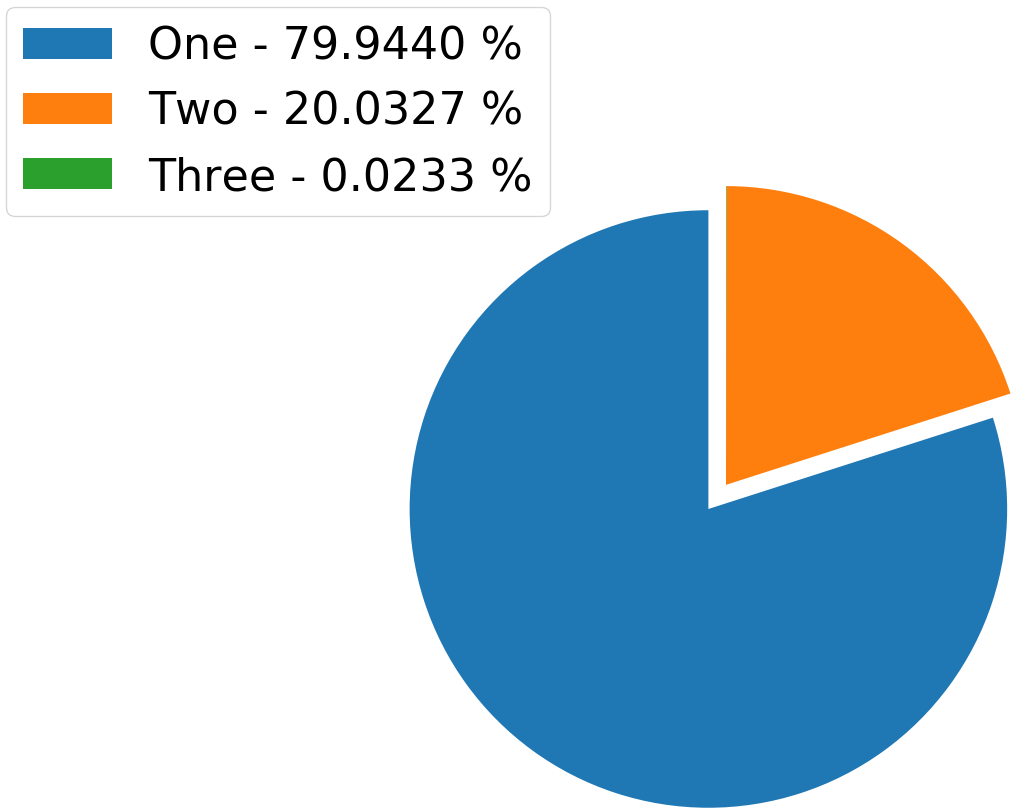
\includegraphics[width=1\linewidth]{pic/PISC_coarse.png}
    \end{minipage}
  }
  \subfigure[PISC fine]{
    \begin{minipage}[t]{0.45\linewidth}
      \centering
      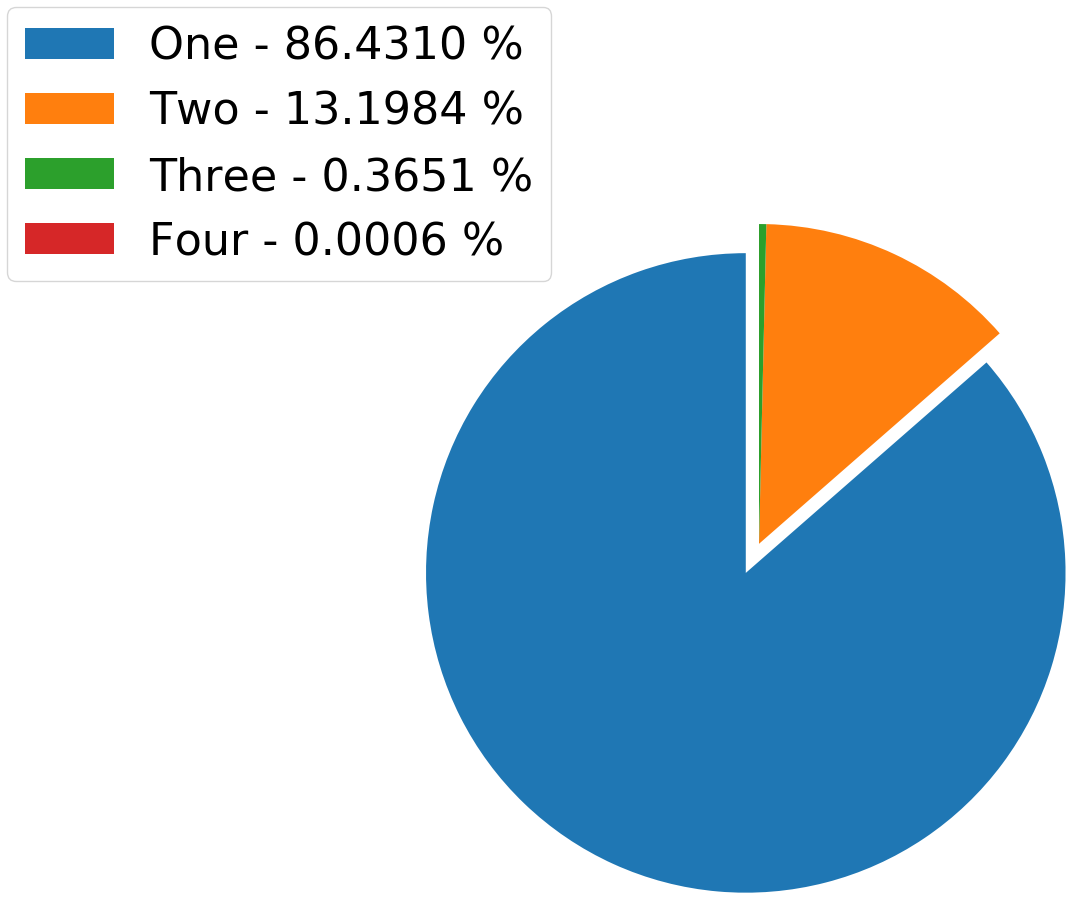
\includegraphics[width=1\linewidth]{pic/PISC_fine.png}
    \end{minipage}
  }
  \subfigure[PIPA-relation 16]{
    \begin{minipage}[t]{0.45\linewidth}
      \centering
      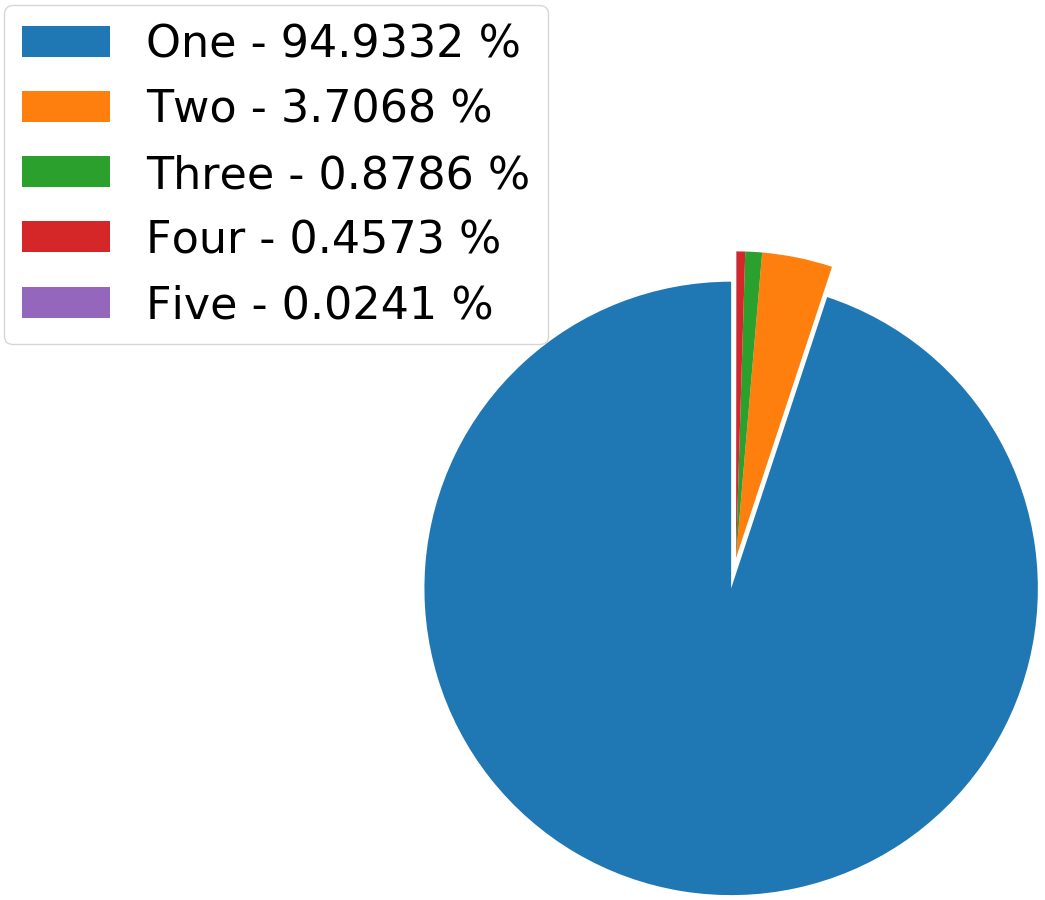
\includegraphics[width=1\linewidth]{pic/PIPA_fine.png}
    \end{minipage}
  }
  % \includegraphics[width=0.8\linewidth]{name.ext}
  \caption{Social relaion categories per image on PISC and PIPA-relation.}
  \label{fig:dataset_analysis}
\end{figure}


In this subsection, we made an analysis on PISC and PIPA-relation. Here we only used its train set and test set for statistic. As shown in Figure \ref{fig:dataset_analysis}, we first calculated the social relation categories of each image, and found almost all images have only one social relation category, and the other half have two categories. For example, on PISC, approximately 79.944\% of images have only one coarse category, while 20.0327\% images have two coarse one.

\subsection{Comparisons with State-of-the-Art Methods}

\begin{table*}[htpb]
  \centering
  \caption{Recall-per-class and mean average precision (mAP) evaluating our PRN model and previous methods on PISC (in \%).}
  \label{tab:pisc_table}
  \begin{tabular}{c|p{0.5cm}<{\centering}|p{0.5cm}<{\centering}|p{0.5cm}<{\centering}|p{0.5cm}<{\centering}||p{0.5cm}<{\centering}|p{0.5cm}<{\centering}|p{0.5cm}<{\centering}|p{0.5cm}<{\centering}|p{0.5cm}<{\centering}|p{0.5cm}<{\centering}|p{0.5cm}<{\centering}}
    \hline
    \multirow{2}{*}{Methods} & \multicolumn{4}{c|}{Coarse relationships} & \multicolumn{7}{|c}{Fine relationships} \\
    \cline{2-12}
    ~ & \rotatebox[origin=l]{90}{Intimate} & \rotatebox[origin=l]{90}{Non-Intimate} & \rotatebox[origin=l]{90}{No Relation} & \rotatebox[origin=l]{90}{mAP} & \rotatebox[origin=l]{90}{Friends} & \rotatebox[origin=l]{90}{Family} & \rotatebox[origin=l]{90}{Couple} & \rotatebox[origin=l]{90}{Professional} & \rotatebox[origin=l]{90}{Commerical} & \rotatebox[origin=l]{90}{No Relation} & \rotatebox[origin=l]{90}{mAP} \\
    \hline\hline
    Union CNN \cite{DBLP:conf/eccv/LuKBL16} & 72.1 & 81.8 & 19.2 & 58.4 & 29.9 & 58.5 & 70.7 & 55.4 & 43.0 & 19.6 & 43.5 \\
    Pair CNN \cite{DBLP:conf/iccv/LiWZK17} & 70.3 & 80.5 & 38.8 & 65.1 & 30.2 & 59.1 & 69.4 & 57.5 & 41.9 & 34.2 & 48.2 \\
    Pair CNN + BBox + Union \cite{DBLP:conf/iccv/LiWZK17} & 71.1 & 81.2 & 57.9 & 72.2 & 32.5 & 62.1 & 73.9 & 61.4 & 46.0 & 52.1 & 56.9 \\
    Pair CNN + BBox + Global \cite{DBLP:conf/iccv/LiWZK17} & 70.5 & 80.0 & 53.7 & 70.5 & 32.2 & 61.7 & 72.6 & 60.8 & 44.3 & 51.0 & 54.6 \\
    Dual-glance \cite{DBLP:conf/iccv/LiWZK17} & 73.1 & \textbf{84.2} & 59.6 & 79.7 & 35.4 & \textbf{68.1} & 76.3 & 70.3 & 57.6 & 60.9 & 63.2 \\
    GRM \cite{DBLP:conf/ijcai/WangCRYCL18} & 81.7 & 73.4 & 65.5 & \textbf{82.8} & 59.6 & 64.4 & \textbf{58.6} & 76.6 & 39.5 & 67.7 & 68.7 \\
    \hline
    Ours & \textbf{81.9} & 67.3 & \textbf{74.7} & 81.8 & \textbf{61.0} & 67.1 & 56.2 & \textbf{76.9} & \textbf{46.0} & \textbf{68.1} & \textbf{69.7} \\
    \hline
  \end{tabular}
\end{table*}

\begin{table}[htpb]
  \centering
  \caption{Accuracy (in \%) evaluating our PRN model and previous methods on PIPA-relation.}
  \label{tab:pipa_table}
  \begin{tabular}{c|c}
    \hline
    Methods & accuracy \\
    \hline\hline
    Two stream CNN \cite{DBLP:conf/cvpr/ZhangPTFB15} & 57.2 \\
    Dual-Glance \cite{DBLP:conf/iccv/LiWZK17} & 59.6 \\
    GRM \cite{DBLP:conf/ijcai/WangCRYCL18} & 62.3 \\
    \hline
    Ours & \textbf{64.7}\\
    \hline
  \end{tabular}
\end{table}

We compare our proposed model with existing state-of-the-art methods on both PISC and PIPA-Relation datasets.Formally, the compared methods are as followed:

\subsubsection{Performance On the PISC dataset}

{\bf UnionCNN}  Following \cite{DBLP:conf/eccv/LuKBL16}, it generates a single CNN model to predicate relations. In this task, we also feeds the union region of person pair to s single CNN for classification.\\
{\bf Pair CNN}\cite{DBLP:conf/iccv/LiWZK17} consists of two equivalent CNNs with shared weights to extracted features for image for two individuals.\\
{\bf Pair CNN + BBox + Union}\cite{DBLP:conf/iccv/LiWZK17} incorporates spatial location information of two bounding box that based the previous pair CNN and Union CNN.\\
{\bf Dual-glance}\cite{DBLP:conf/iccv/LiWZK17} implements coarse and fine prediction which includes three and six relationships. Dual-glance employing pair CNN + BBox + BBox + Union and utilized surrounding region proposal to refine the prediction.\\
{\bf GRM}\cite{DBLP:conf/ijcai/WangCRYCL18} propse a graph reasoning model that unifies the frequence of co-concurrences of each relationship-object pair to facilitate social relation.

Similar to the model of GRM, we also adopt the per-class recall and mean average precision(mAP) to evaluate our model. The experiments data are reported in Table 1. First, both Pair CNN + BBox + Union, Pair CNN + BBox + Global, Dual-glance are incur extra Faster-RCNN\cite{DBLP:conf/nips/RenHGS15} to extract the local contextual cues(object proposal). GRM utilized the object proposal to construct a semantic-aware  knowledge graph for reason about the social relationship. It is notable that both of them incur extra detection annotations that contains noisies.Specifically, our model achieves an accuracy of 75.0\% and mAP of 82.1\% for the coarse-level recognition. the model also takes an accuracy of 65.6\% and mAP of 69.7\% for the fine-level dataset, our model beating previous best model in the fine-level recognition ,but slightly lower on coarse-level than the best model before.

\subsubsection{Performance on the PIPA-Relation Dataset}

On this dataset, we also compare our proposed model with the existing methods,i.e, Two stream CNN\cite{DBLP:conf/cvpr/SunSF17},Dual-glance\cite{DBLP:conf/iccv/LiWZK17} and GRM\cite{DBLP:conf/ijcai/WangCRYCL18} that achieves the best performance before. Specifically, we directly reprint the experimental of serveral baselines from the literature. The result are presented in Table 2. Notably, our PRN significantly outperforms previous methods. Still, our model outperforms all the baselines in PIPA-relation, and beating the best of them 2.4\%.  

\subsection{Analysis on Experimental Result}

\begin{table}[htb] 
	\vspace*{-7.5pt}
	\centering
	\caption{The mAP and accuracy result of RCNN, our model and our model with contexual region that implements in the same way as dual-glance (in \%)}
	\vspace*{0.1cm}
	\scalebox{1}{
		\begin{tabular}{c|c|c|c|c}
			\toprule
			\multirow{2}{*}{Methods} &
			\multicolumn{2}{c|}{PISC coarse} &
			\multicolumn{2}{|c}{PISC fine}  \\
 				 & accuracy & mAP & accuracy & mAP  \\
			\midrule
			Ours(max) & 74.3 & 80.8 & 64.1 & 68.3 \\
			\midrule
			Ours(average) & 74.6 & 80.1 & 63.8 & 68.3 \\
			\midrule
			Ours(atten) & \textbf{75.1} & \textbf{81.8} & \textbf{65.7} & \textbf{69.7} \\
			\midrule
			Ours(atten)+region & 74.9 & 81.2 & 65.3 & 69.1 \\
			\midrule
		\end{tabular}
	}
\end{table}

In this section, we first present the comparison result  of message passing mechanism and analsis the reasons behind, and the result present in Table 3.
Then, we conduct a conditional experiment to investigate the effectiveness of 
the factor of region contexuals and the interaction between person-pair.

\subsubsection{Significance of message passing}

In our framework, the core component is the introduction of message passing mechanism, and one of the key component is the message pooling functions that use learnt weights sum to aggregate hidden state of other relation nodes into message. To futher inverstigate the improvement of our approach on recognizing social relationships, we evaluate variants of our model
with standard pooling methods. The first is to use average-pooling (avg. pool) instead of the learnt weighted sum to
aggregate the hidden states. The second is similar to the first
one, but uses max-pooling (max pool).

\begin{figure*}[ht]
  \centering
  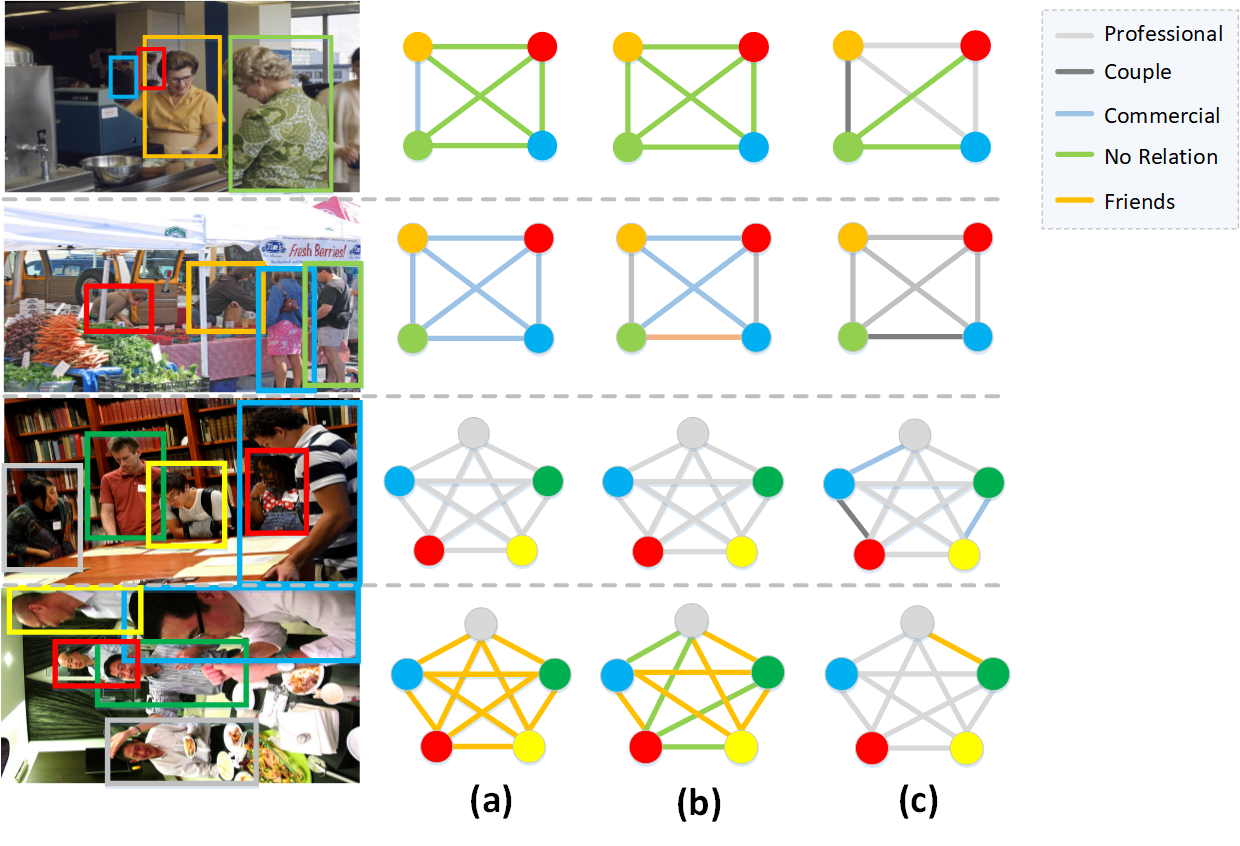
\includegraphics[width=0.9\linewidth]{pic/case_study_pisc_fine_union.png}
  \caption{Comparison of social relation graphs from different sources: (a) PISC fine, (b) our PRN and (c) GRM. People with boxes of various colors on the original image correspond to the same color node on right of the image. An edge linked to two nodes represents the social relationships between them and its meaning can be found in the right legend. From these example, all edges in (a) are almost identical, which suggests that the social relationships in a still image are always stable.}
  \label{fig:case_study}
\end{figure*}

\subsubsection{Analysis of contextual information}

First, our model is to process the cue of contexual of relationships without contextual object region that incured in Dual-glance and GRM by extra detecion annotation. 
From the object regions point of view, the effect of object regions is provide the information of scene to constraint the vector of the relationship and the information of scene is single. So, object regions is limited for the images with multi-class social relationship. But, the information of contexual relationships is different, and it is more appropriate for the fine relationships.
For example, if the object of laptop is useful to classifier the relationship as professional that is not contribute to the relationship of friend.
As tabel 3 reported, the model of RCNN is the lowest, and
 \cite{DBLP:conf/iccv/LiWZK17} trained a model with attention machanisms to exploit different object regions cues according different pairs of people. we also conduct a attention machanisms as same as Dual-glance, but the performance do not improved as reported in Table 3. 
One possible reason is that the object regions cues is coverd by contexual information of relationships cues, and the result of experiments proved the analysis before. 

%\subsection{Ablation Study}

\subsection{Case Study}\label{section:cs}

Three examples in Figure \ref{fig:case_study} are shown to illustrate the ability of our PRN to infer social relationshps. We compared two predicted social relationships, one from our PRN and the another from GRM \cite{DBLP:conf/ijcai/WangCRYCL18}. We found that compared to the social relation graphs in (c), the graphs in (b) are very similar to the graphs in (a), which means that our PRN performs better than GRM. In addition, the edges in (a) are almost identical, meaning the social relationship in a still image are almost always stable. More importantly, similar to (a), over half of the edges in (b) are identical, which strongly suggests that the contextual relationship cues are very significant for social relationship understanding and our PRN can fully utilize it. Considering the first example, the true social relation between the person in an orange box and another in a green one is No Relation, which can be correctly predicted by our PRN while being incorrectly predicted as Couple by GRM, and the accuracy of PRN is 100\% while 33.3\% in GRM.

\section{Conclusion}
% This part will be written by {\bf liangjinrui}.
In this study, we propse a person-pair relation network(PRN) that aims to solve social relationship recognition of an image. The proposed model incoporates the information of contexual relationships. The key challenge is to design a model for interaction between social relationships. PRN consists of a reasoning module that propagates relationship message through the RNNs. PRN adopt message passing to finish the reasoning of the social relationships in an image. In this way, it improves the quality of relationps prediction. Specifically, a attention also utilized to compute the weights factor for the connected nodes in a social graph, and these weights introduced to aggregates the messages. We also analysis the influence of contexual relationships and contexual object region, and we found that the cue of contexual object region coverd by contexual relationships. Extensive experiments on two large-scale benchmarks(PISC and PIPA-Relation) achieves better performance  without incur extra detecion annotations.

\newpage
%% The file named.bst is a bibliography style file for BibTeX 0.99c
\bibliographystyle{named}
\bibliography{ijcai19}

\end{document}
